\chapter{Elektronenschillen en het periodiek systeem}\label{ch:g10:electron-shells}

Neon gloeit roodoranje in een lichtreclame; natrium, een zacht \omterm{def:g9:periodic-table-first-look:metal}{metaal},
vliegt in brand in water; chloor is een verstikkend geelgroen gas. Toch
verschillen hun \omterm{def:g7:atoms-and-molecules:atom}{atomen} maar één of twee \omterm{def:g9:inside-the-atom:proton}{protonen}: neon heeft er 10,
natrium 11, chloor 17. Waarom zouden buren in het \omterm{def:g9:periodic-table-first-look:periodic-table}{periodiek systeem} zich
zo verschillend gedragen, terwijl natrium en kalium, die qua \omterm{def:g9:inside-the-atom:atomic-number}{atoomnummer}
ver uit elkaar liggen, zich zo gelijk gedragen? Het antwoord zit in de
manier waarop de \omterm{def:g9:inside-the-atom:nucleus}{elektronen} van een \omterm{def:g7:atoms-and-molecules:atom}{atoom} gerangschikt zijn.

\begin{recall}
Een \omterm{def:g7:atoms-and-molecules:atom}{atoom} heeft $Z$ \omterm{def:g9:inside-the-atom:proton}{protonen} in zijn kern en, als het neutraal is, $Z$
\omterm{def:g9:inside-the-atom:nucleus}{elektronen} eromheen (\cref{ch:g9:inside-the-atom}). Het \omterm{def:g9:periodic-table-first-look:periodic-table}{periodiek systeem}
ordent de elementen naar $Z$ in perioden (rijen) en groepen (kolommen);
de elementen van een groep gedragen zich hetzelfde
(\cref{ch:g9:periodic-table-first-look}). \omterm{def:g7:atoms-and-molecules:atom}{Atomen} nemen \omterm{def:g9:inside-the-atom:nucleus}{elektronen} op of
staan ze af en worden zo \omterm{def:g9:ions:ion}{ionen} (\cref{ch:g9:ions}).
\end{recall}

\section{Elektronenconfiguratie}

\begin{definition}[Schillen, subschillen en elektronenconfiguratie]\label{def:g10:electron-shells:configuration}
De \omterm{def:g9:inside-the-atom:nucleus}{elektronen} van een \omterm{def:g7:atoms-and-molecules:atom}{atoom} zijn verdeeld over \emph{schillen}\index{schil},
genummerd $n = 1, 2, 3, \ldots$ van de kern naar buiten; hoe hoger $n$,
hoe verder van de kern en hoe minder sterk de \omterm{def:g9:inside-the-atom:nucleus}{elektronen} vastgehouden
worden. Elke schil is verdeeld in \emph{subschillen}\index{subschil} die
een letter als naam hebben: schil 1 heeft een s-subschil (1s), schil 2
een s- en een p-subschil (2s, 2p), schil 3 heeft 3s en 3p (en 3d, die
later aan bod komt). Een s-subschil bevat hoogstens 2 \omterm{def:g9:inside-the-atom:nucleus}{elektronen}, een
p-subschil hoogstens 6. De
\emph{elektronenconfiguratie}\index{elektronenconfiguratie} van een \omterm{def:g7:atoms-and-molecules:atom}{atoom}
somt de bezette subschillen op met hun aantal \omterm{def:g9:inside-the-atom:nucleus}{elektronen} als exponent:
$1\mathrm{s}^2\,2\mathrm{s}^2\,2\mathrm{p}^4$ voor zuurstof.
\end{definition}

\begin{method}[Een elektronenconfiguratie opschrijven, tot $Z = 20$]\label{met:g10:electron-shells:write}
\begin{enumerate}
  \item Tel de \omterm{def:g9:inside-the-atom:nucleus}{elektronen}: $Z$ voor een neutraal \omterm{def:g7:atoms-and-molecules:atom}{atoom}.
  \item Vul de \omterm{def:g10:electron-shells:configuration}{subschillen} in deze volgorde, elk tot het maximum voordat
        je aan de volgende begint:
        \[
          1\mathrm{s} \to 2\mathrm{s} \to 2\mathrm{p} \to 3\mathrm{s} \to
          3\mathrm{p} \to 4\mathrm{s}.
        \]
  \item Controleer dat de exponenten samen het aantal \omterm{def:g9:inside-the-atom:nucleus}{elektronen} geven.
\end{enumerate}
Natrium, $Z = 11$: $1\mathrm{s}^2\,2\mathrm{s}^2\,2\mathrm{p}^6\,3\mathrm{s}^1$.
Chloor, $Z = 17$: $1\mathrm{s}^2\,2\mathrm{s}^2\,2\mathrm{p}^6\,3\mathrm{s}^2\,3\mathrm{p}^5$.
Calcium, $Z = 20$: $1\mathrm{s}^2\,2\mathrm{s}^2\,2\mathrm{p}^6\,3\mathrm{s}^2\,3\mathrm{p}^6\,4\mathrm{s}^2$.
\end{method}

\begin{omfigure}
\begin{tikzpicture}[font=\small, y=0.95cm]
  \draw[->, black!60] (-0.4,0) -- (-0.4,5.4) node[above, align=center, font=\footnotesize]
    {verder van\\ de kern};
  \foreach \y/\lab/\n/\x in {0.3/1s/2/0.5, 1.3/2s/2/0.5, 1.9/2p/6/2.4, 3.0/3s/2/0.5,
      3.6/3p/6/2.4, 4.4/4s/2/0.5} {
    \foreach \k in {1,...,\n} \draw[omDef, fill=omDef!10] (\x+0.42*\k-0.42,\y) rectangle ++(0.36,0.36);
    \node[anchor=east] at (\x-0.05,\y+0.18) {\lab};
  }
  \node[anchor=west, font=\footnotesize] at (5.3,0.48) {schil 1: hoogstens 2 elektronen};
  \node[anchor=west, font=\footnotesize] at (5.3,1.7) {schil 2: $2 + 6 = 8$};
  \node[anchor=west, font=\footnotesize] at (5.3,3.4) {schil 3: $2 + 6 = 8$ (tot $Z = 18$)};
  \node[anchor=west, font=\footnotesize] at (5.3,4.58) {4s vult zich vóór 3d};
\end{tikzpicture}

{\small De volgorde van opvullen, tot $Z = 20$. Elk vakje is een plaats
voor één \omterm{def:g9:inside-the-atom:nucleus}{elektron}: een \omterm{def:g10:electron-shells:configuration}{s-subschil} heeft 2 plaatsen, een \omterm{def:g10:electron-shells:configuration}{p-subschil} 6.}
\end{omfigure}

\section{Valentie-elektronen}

\begin{definition}[Valentie- en rompelektronen]\label{def:g10:electron-shells:valence}
De \omterm{def:g9:inside-the-atom:nucleus}{elektronen} in de buitenste bezette \omterm{def:g10:electron-shells:configuration}{schil} (de \omterm{def:g10:electron-shells:configuration}{schil} met de hoogste $n$)
zijn de \emph{valentie-elektronen}\index{valentie-elektron}; de andere
zijn de \emph{rompelektronen}\index{rompelektron}. Alleen de
\omterm{def:g9:inside-the-atom:nucleus}{valentie-elektronen} doen mee aan \omterm{def:g7:chemical-reactions:reaction}{chemische reacties}.
\end{definition}

\begin{example}[Valentie-elektronen tellen]\label{ex:g10:electron-shells:count}
Zuurstof, $1\mathrm{s}^2\,2\mathrm{s}^2\,2\mathrm{p}^4$: buitenste \omterm{def:g10:electron-shells:configuration}{schil} $n =
2$, $2 + 4 = 6$ \omterm{def:g10:electron-shells:valence}{valentie-elektronen}. Natrium, $\ldots 3\mathrm{s}^1$: 1
\omterm{def:g10:electron-shells:valence}{valentie-elektron}. Chloor, $\ldots 3\mathrm{s}^2\,3\mathrm{p}^5$: 7.
Neon, $1\mathrm{s}^2\,2\mathrm{s}^2\,2\mathrm{p}^6$: 8, een volle \omterm{def:g10:electron-shells:configuration}{schil}.
\end{example}

\section{De tabel opnieuw opgebouwd uit configuraties}

\begin{proposition}[Periode en groep uit de configuratie]\label{prop:g10:electron-shells:table}
Voor de elementen tot $Z = 20$ geldt:
\begin{itemize}
  \item de periode van een element is het nummer $n$ van zijn buitenste
        \omterm{def:g10:electron-shells:configuration}{schil};
  \item elementen van eenzelfde groep hebben evenveel \omterm{def:g10:electron-shells:valence}{valentie-elektronen}
        --- één in \omterm{def:g9:periodic-table-first-look:period}{groep} 1, twee in \omterm{def:g9:periodic-table-first-look:period}{groep} 2, drie tot acht in de \omterm{def:g9:periodic-table-first-look:period}{groepen} 13
        tot en met 18 (helium, met 2, is een uitzondering).
\end{itemize}
De twee linkerkolommen, waar de laatste \omterm{def:g9:inside-the-atom:nucleus}{elektronen} in een \omterm{def:g10:electron-shells:configuration}{s-subschil}
komen, vormen het s-blok; de \omterm{def:g9:periodic-table-first-look:period}{groepen} 13 tot en met 18 vormen het
p-blok.
\end{proposition}

\begin{omfigure}
\omperiodictable[upto=20, f block=false, cell=0.86cm, colour=blocks, legend=true,
  values={H/1,He/2,Li/2.1,Be/2.2,B/2.3,C/2.4,N/2.5,O/2.6,F/2.7,Ne/2.8,
    Na/2.8.1,Mg/2.8.2,Al/2.8.3,Si/2.8.4,P/2.8.5,S/2.8.6,Cl/2.8.7,Ar/2.8.8,
    K/2.8.8.1,Ca/2.8.8.2}]

{\small De eerste twintig elementen, met het aantal \omterm{def:g9:inside-the-atom:nucleus}{elektronen} in elke
\omterm{def:g10:electron-shells:configuration}{schil} onder het symbool ($2.8.1$ voor natrium: 2 in \omterm{def:g10:electron-shells:configuration}{schil} 1, 8 in \omterm{def:g10:electron-shells:configuration}{schil} 2,
1 in \omterm{def:g10:electron-shells:configuration}{schil} 3). De kleuren geven het s- en het p-blok aan.}
\end{omfigure}

\section{Families}

\begin{definition}[Chemische families]\label{def:g10:electron-shells:family}
Een \emph{chemische familie}\index{chemische familie} is een groep van het
\omterm{def:g9:periodic-table-first-look:periodic-table}{periodiek systeem} waarvan de elementen hun belangrijkste chemische
eigenschappen delen. Drie families hebben een naam: de
\emph{alkalimetalen}\index{alkalimetaal} (\omterm{def:g9:periodic-table-first-look:period}{groep} 1 zonder waterstof:
lithium, natrium, kalium\dots), zachte \omterm{def:g9:periodic-table-first-look:metal}{metalen} die heftig met water
reageren; de \emph{halogenen}\index{halogeen} (\omterm{def:g9:periodic-table-first-look:period}{groep} 17: fluor, chloor,
broom, jood), gekleurde, reactieve \omterm{def:g9:periodic-table-first-look:metal}{niet-metalen}; en de
\emph{edelgassen}\index{edelgas} (\omterm{def:g9:periodic-table-first-look:period}{groep} 18: helium, neon, argon\dots), die
met bijna niets reageren.
\end{definition}

\begin{proposition}[Waarom een familie zich hetzelfde gedraagt]\label{prop:g10:electron-shells:why}
De elementen van een familie hebben evenveel \omterm{def:g10:electron-shells:valence}{valentie-elektronen}, en
chemie is de zaak van de \omterm{def:g10:electron-shells:valence}{valentie-elektronen}: lithium, natrium en kalium
hebben er allemaal één, de halogenen zeven, de \omterm{def:g10:electron-shells:family}{edelgassen} een volle
buitenste \omterm{def:g10:electron-shells:configuration}{schil}.
\end{proposition}

\begin{omfigure}
\omperiodictable[colour=families, legend=true, cell=0.86cm, f block=false]

{\small Families van het \omterm{def:g9:periodic-table-first-look:periodic-table}{periodiek systeem}: \omterm{def:g10:electron-shells:family}{alkalimetalen},
aardalkalimetalen (\omterm{def:g9:periodic-table-first-look:period}{groep} 2), \omterm{def:g10:electron-shells:family}{halogenen} en \omterm{def:g10:electron-shells:family}{edelgassen}.}
\end{omfigure}

\begin{omfigure}
\begin{minipage}[b]{0.48\linewidth}\centering
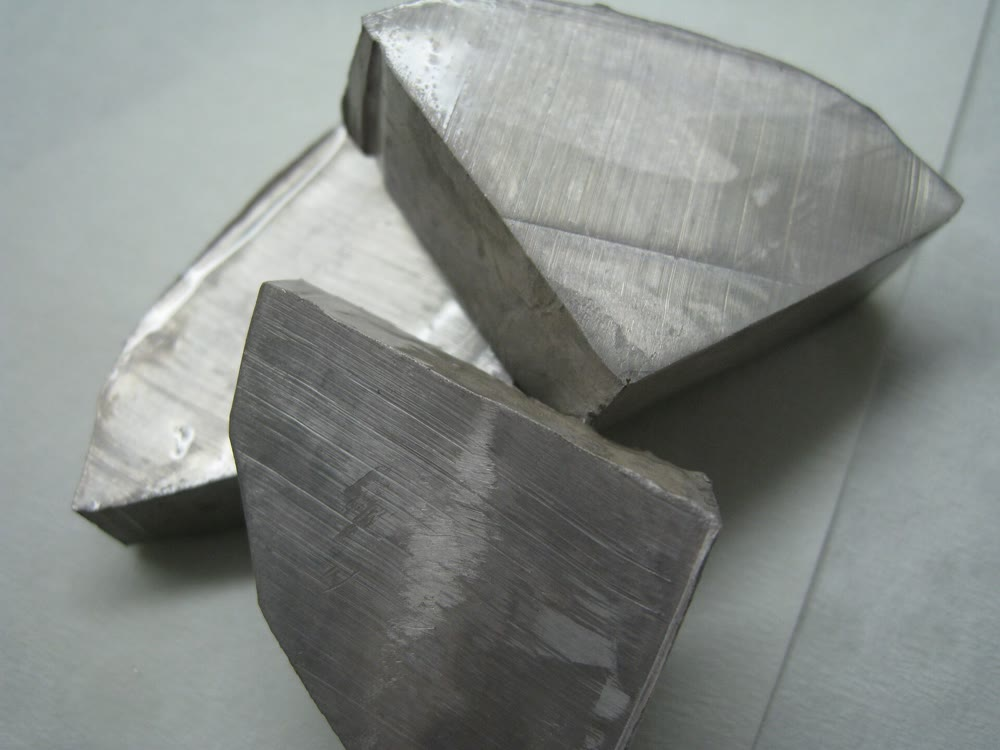
\includegraphics[width=\linewidth,height=4.4cm,keepaspectratio]{images/book1/sodium.jpg}

{\small Natrium, een \omterm{def:g10:electron-shells:family}{alkalimetaal}, gesneden met een mes: vers is het
zacht en zilverig, aan de \omterm{def:g4:air-a-mixture-of-gases:air}{lucht} wordt het meteen dof. Foto: Dnn87,
CC BY-SA 3.0.}
\end{minipage}\hfill
\begin{minipage}[b]{0.48\linewidth}\centering
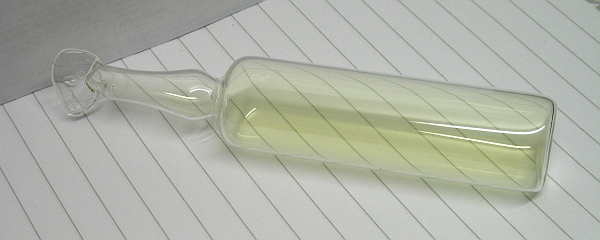
\includegraphics[width=\linewidth,height=4.4cm,keepaspectratio]{images/book1/chlorine-ampoule.jpg}

{\small Chloor, een \omterm{def:g10:electron-shells:family}{halogeen}: een geelgroen gas, hier ingesloten in een
glazen ampul. Foto: W.~Oelen, CC BY-SA 3.0.}
\end{minipage}
\end{omfigure}

\begin{inthelab}[Natrium in water]
Achter een scherm laat de docent een stukje natrium zo groot als een
rijstkorrel in een grote kom water vallen. Het drijft, smelt tot een
glanzend bolletje en schiet sissend rond tot het verdwenen is; het gas
dat vrijkomt is waterstof, en het water dat overblijft is basisch.
\end{inthelab}

\begin{safety}{\ghs[0.75cm]{GHS02}\ghs[0.75cm]{GHS05}\quad\ghs[0.75cm]{GHS03}\ghs[0.75cm]{GHS06}}
% ledger: ghs:Na, ghs:Cl2
Natrium: geeft met water ontvlambaar waterstof af (GHS02), veroorzaakt
ernstige brandwonden (GHS05). Chloor: een oxiderend gas (GHS03), giftig
bij inademing (GHS06), ook irriterend en zeer giftig voor in het water
levende organismen. Beide worden alleen door de docent gehanteerd.
\end{safety}

\section{Stabiele ionen en de edelgasregel}

\begin{definition}[Duet- en octetregel]\label{def:g10:electron-shells:octet}
De \omterm{def:g10:electron-shells:family}{edelgassen}, met een volle buitenste \omterm{def:g10:electron-shells:configuration}{schil}, reageren nauwelijks: hun
configuratie is bijzonder stabiel. Als \omterm{def:g7:atoms-and-molecules:atom}{atomen} van de eerste elementen
\omterm{def:g9:ions:ion}{ionen} vormen, nemen ze \omterm{def:g9:inside-the-atom:nucleus}{elektronen} op of staan ze er af om de
configuratie van het dichtstbijzijnde \omterm{def:g10:electron-shells:family}{edelgas} te bereiken: twee
\omterm{def:g9:inside-the-atom:nucleus}{elektronen} in \omterm{def:g10:electron-shells:configuration}{schil} 1, zoals helium, voor de lichtste \omterm{def:g7:atoms-and-molecules:atom}{atomen} --- de
\emph{duetregel}\index{duetregel} --- en acht \omterm{def:g9:inside-the-atom:nucleus}{elektronen} in de buitenste
\omterm{def:g10:electron-shells:configuration}{schil}, zoals neon of argon, voor de andere --- de
\emph{octetregel}\index{octetregel}.
\end{definition}

\begin{example}[Ionen voorspeld door de regel]\label{ex:g10:electron-shells:ions}
Natrium, $2.8.1$, staat zijn enige \omterm{def:g10:electron-shells:valence}{valentie-elektron} af: \ce{Na+}, $2.8$,
zoals neon. Magnesium, $2.8.2$, staat er twee af: \ce{Mg^{2+}}.
Aluminium, $2.8.3$, staat er drie af: \ce{Al^{3+}}. Chloor, $2.8.7$, neemt
er één op: \ce{Cl-}, $2.8.8$, zoals argon. Zuurstof, $2.6$, neemt er twee
op: \ce{O^{2-}}. Zwavel, $2.8.6$: \ce{S^{2-}}. Lithium, $2.1$, staat er één
af en houdt $2$ over, zoals helium: \ce{Li+}.
\end{example}

\begin{omfigure}
\begin{tikzpicture}[font=\small]
  \foreach \x/\nm/\cfg/\col in {0/{Na}/{$1\mathrm{s}^2\,2\mathrm{s}^2\,2\mathrm{p}^6\,3\mathrm{s}^1$}/omDef,
      5.8/{\ce{Na+}}/{$1\mathrm{s}^2\,2\mathrm{s}^2\,2\mathrm{p}^6$}/omProp,
      11.0/{Ne}/{$1\mathrm{s}^2\,2\mathrm{s}^2\,2\mathrm{p}^6$}/gray} {
    \node[draw=\col, fill=\col!6, rounded corners=2pt, align=center, text width=3.4cm]
      at (\x,0) {\textbf{\nm}\\ \cfg};
  }
  \draw[->, thick, omProp] (2.0,0) -- (3.8,0) node[midway, above, font=\footnotesize] {staat 1 \ce{e-} af};
  \node at (8.4,0) {$=$};
  \node[font=\footnotesize, align=center] at (8.4,-0.75) {dezelfde\\ configuratie};
\end{tikzpicture}

{\small Het natriumion heeft de configuratie van neon, het dichtstbijzijnde
\omterm{def:g10:electron-shells:family}{edelgas}.}
\end{omfigure}

\begin{remark}[Grenzen van de regel]\label{rem:g10:electron-shells:limits}
De regel werkt goed voor de eerste twintig elementen en hun eenvoudige
\omterm{def:g9:ions:ion}{ionen}. Veel elementen, zoals ijzer (\ce{Fe^{2+}} en \ce{Fe^{3+}}), volgen
hem niet; de redenen, en een betere beschrijving van \omterm{def:g9:inside-the-atom:nucleus}{elektronen}, staan in
het deel voor het eerste jaar aan de universiteit.
\end{remark}

\section{Oefeningen}

\begin{exercise}[$\star$]\label{exo:g10:electron-shells:1}
Schrijf de \omterm{def:g10:electron-shells:configuration}{elektronenconfiguraties} op van koolstof ($Z = 6$), stikstof
($Z = 7$) en magnesium ($Z = 12$).
\end{exercise}

\begin{exercise}[$\star$]\label{exo:g10:electron-shells:2}
Hoeveel \omterm{def:g10:electron-shells:valence}{valentie-elektronen} hebben koolstof, stikstof en magnesium?
\end{exercise}

\begin{exercise}[$\star$]\label{exo:g10:electron-shells:3}
In welke periode en welke groep staat het element met configuratie
$1\mathrm{s}^2\,2\mathrm{s}^2\,2\mathrm{p}^6\,3\mathrm{s}^2\,3\mathrm{p}^3$?
\end{exercise}

\begin{exercise}[$\star$]\label{exo:g10:electron-shells:4}
Noem de drie families van dit hoofdstuk en geef van elk twee elementen.
\end{exercise}

\begin{exercise}[$\star$]\label{exo:g10:electron-shells:5}
Formuleer de \omterm{def:g10:electron-shells:octet}{octetregel}.
\end{exercise}

\begin{exercise}[$\star\star$]\label{exo:g10:electron-shells:6}
Geef met de edelgasregel het \omterm{def:g9:ions:ion}{ion} dat kalium ($Z = 19$) vormt en het \omterm{def:g9:ions:ion}{ion}
dat fluor ($Z = 9$) vormt, met hun configuraties.
\end{exercise}

\begin{exercise}[$\star\star$]\label{exo:g10:electron-shells:7}
Een element heeft 2 \omterm{def:g9:inside-the-atom:nucleus}{elektronen} in zijn derde \omterm{def:g10:electron-shells:configuration}{schil}, en de derde \omterm{def:g10:electron-shells:configuration}{schil} is
zijn buitenste \omterm{def:g10:electron-shells:configuration}{schil}. Geef zijn configuratie, zijn \omterm{def:g9:inside-the-atom:atomic-number}{atoomnummer} en zijn
naam.
\end{exercise}

\begin{exercise}[$\star\star$]\label{exo:g10:electron-shells:8}
Schrijf met stabiele \omterm{def:g9:ions:ion}{ionen} de formule op van de \omterm{def:g9:ions:ionic-compound}{ionverbinding} van
magnesium en chloor, en daarna van die van aluminium en zuurstof.
\end{exercise}

\begin{exercise}[$\star\star$]\label{exo:g10:electron-shells:9}
Kijk naar de tabel van de eerste twintig elementen. Welke elementen
hebben evenveel \omterm{def:g10:electron-shells:valence}{valentie-elektronen} als zuurstof?
\end{exercise}

\begin{exercise}[$\star\star$]\label{exo:g10:electron-shells:10}
Waarom vormt neon, anders dan natrium en chloor, bij \omterm{def:g7:chemical-reactions:reaction}{chemische reacties}
geen \omterm{def:g9:ions:ion}{ionen}?
\end{exercise}

\begin{exercise}[$\star\star$]\label{exo:g10:electron-shells:11}
Het \omterm{def:g9:ions:ion}{ion} \ce{X^{2+}} heeft de configuratie van argon. Bepaal $X$.
\end{exercise}

\begin{exercise}[$\star\star\star$]\label{exo:g10:electron-shells:12}
Helium heeft 2 \omterm{def:g10:electron-shells:valence}{valentie-elektronen} maar staat in \omterm{def:g9:periodic-table-first-look:period}{groep} 18, niet in
\omterm{def:g9:periodic-table-first-look:period}{groep} 2. Leg uit met zijn configuratie.
\end{exercise}

\begin{exercise}[$\star\star\star$]\label{exo:g10:electron-shells:13}
Kalium reageert nog heftiger met water dan natrium. Bedenk een verklaring
met de afstand van het \omterm{def:g10:electron-shells:valence}{valentie-elektron} tot de kern.
\end{exercise}

\begin{exercise}[$\star\star\star$]\label{exo:g10:electron-shells:14}
Geef de configuraties van \ce{S^{2-}}, \ce{Cl-}, \ce{K+} en
\ce{Ca^{2+}}. Wat hebben ze gemeen?
\end{exercise}

\begin{exercise}[$\star\star\star$]\label{exo:g10:electron-shells:15}
Een element uit periode 3 vormt het \omterm{def:g9:ions:ion}{ion} \ce{Y^{3-}}. Bepaal zijn groep,
zijn configuratie en zijn naam.
\end{exercise}

\section{Probleem: Robijn, saffier en korund}

\begin{problem}[{Weekendprobleem --- de elektronen achter een edelsteen: van
twee configuraties naar het aantal verplaatste elektronen in één gram}]
\label{pb:g10:electron-shells:1}
Robijnen en saffieren zijn edelsteenvormen van korund, een \omterm{def:g9:ions:ionic-compound}{ionverbinding}
van aluminium en zuurstof; een spoortje andere \omterm{def:g9:periodic-table-first-look:metal}{metalen} geeft ze hun
kleur. Korund is hard genoeg om bijna alles te krassen, en korundpoeder
wordt gebruikt om lenzen te polijsten. Neem voor de massa van een \omterm{def:g9:inside-the-atom:proton}{nucleon}
\qty{1.67e-27}{kg}; aluminium-27 heeft 27 \omterm{def:g9:inside-the-atom:proton}{nucleonen}, zuurstof-16 heeft 16.

\medskip
\noindent\textbf{Deel I --- De \omterm{def:g7:atoms-and-molecules:atom}{atomen}.}
\begin{enumerate}
  \item Geef het aantal \omterm{def:g9:inside-the-atom:proton}{protonen} en \omterm{def:g9:inside-the-atom:nucleus}{elektronen} van een aluminiumatoom
        ($Z = 13$) en van een zuurstofatoom ($Z = 8$).
  \item Schrijf hun \omterm{def:g10:electron-shells:configuration}{elektronenconfiguraties} op.
  \item Hoeveel \omterm{def:g10:electron-shells:valence}{valentie-elektronen} heeft elk? In welke periode en groep
        staat elk?
  \item Is aluminium een \omterm{def:g9:periodic-table-first-look:metal}{metaal} of een \omterm{def:g9:periodic-table-first-look:metal}{niet-metaal}? En zuurstof?
\end{enumerate}

\medskip
\noindent\textbf{Deel II --- De \omterm{def:g9:ions:ion}{ionen}.}
\begin{enumerate}[resume]
  \item Welk \omterm{def:g9:ions:ion}{ion} vormt aluminium volgens de \omterm{def:g10:electron-shells:octet}{octetregel}? Schrijf de
        configuratie op.
  \item Welk \omterm{def:g9:ions:ion}{ion} vormt zuurstof? Schrijf de configuratie op.
  \item Welk \omterm{def:g10:electron-shells:family}{edelgas} heeft dezelfde configuratie als beide \omterm{def:g9:ions:ion}{ionen}?
  \item Hoeveel \omterm{def:g9:inside-the-atom:nucleus}{elektronen} staat een aluminiumatoom af, en hoeveel neemt
        een zuurstofatoom op?
\end{enumerate}

\medskip
\noindent\textbf{Deel III --- De formule.}
\begin{enumerate}[resume]
  \item Bepaal de formule van korund, de neutrale verbinding van deze
        \omterm{def:g9:ions:ion}{ionen}.
  \item Hoeveel \omterm{def:g9:inside-the-atom:nucleus}{elektronen} staan de aluminiumatomen in één formule-eenheid
        af? Hoeveel nemen de zuurstofatomen op?
  \item Waarom moeten deze twee aantallen gelijk zijn?
  \item Een robijn bevat een spoortje chroomionen \ce{Cr^{3+}} in plaats
        van sommige \ce{Al^{3+}}. Waarom kan een \ce{Cr^{3+}}-ion de plaats
        van een \ce{Al^{3+}}-ion innemen zonder de ladingen te verstoren?
\end{enumerate}

\medskip
\noindent\textbf{Deel IV --- Eén gram korund.}
\begin{enumerate}[resume]
  \item Hoeveel \omterm{def:g9:inside-the-atom:proton}{nucleonen} zitten er in één formule-eenheid korund?
  \item Bereken de massa van één formule-eenheid (\omterm{def:g9:inside-the-atom:nucleus}{elektronen} verwaarloosd).
  \item Hoeveel formule-eenheden zitten er in \qty{1}{g} korund?
  \item Hoeveel \ce{Al^{3+}}-ionen en \ce{O^{2-}}-ionen zijn dat?
  \item Waarom mag je bij vraag 14 de \omterm{def:g9:inside-the-atom:nucleus}{elektronen} verwaarlozen?
  \item Hoeveel \omterm{def:g9:inside-the-atom:nucleus}{elektronen} zijn er van aluminium naar zuurstof
        overgegaan om \qty{1}{g} korund te maken?
\end{enumerate}
\end{problem}
